\documentclass{beamer}
\usepackage[utf8]{inputenc}
\usepackage[brazil]{babel}
\usepackage{graphicx,hyperref,icmc,url}
\usepackage{multirow}
\usepackage{multimedia}

% The title of the presentation:
%  - first a short version which is visible at the bottom of each slide;
%  - second the full title shown on the title slide;
\title[Trabalho de Conclusão de Curso]{Aplicação de deep learning em dispositivos Android}

% Optional: a subtitle to be dispalyed on the title slide
\subtitle{}

% The author(s) of the presentation:
%  - again first a short version to be displayed at the bottom;
%  - next the full list of authors, which may include contact information;
\author[Tiago de Miranda Leite]{
    \Large{Tiago de Miranda Leite} \\ \medskip
    \small{NUSP: 7595289} \\
    \small{\href{mailto:tiago.miranda.leite@usp.br}{\nolinkurl{tiago.miranda.leite@usp.br}}} \\ \bigskip
    \small{Orientador: Prof. Dr. João do Espírito Santo Batista Neto} \\ \bigskip
    \large{Apresentação do Trabalho de Conclusão de Curso}
}

% The institute:
%  - to start the name of the university as displayed on the top of each slide
%    this can be adjusted such that you can also create a Dutch version
%  - next the institute information as displayed on the title slide
\institute[ICMC/USP]{
    Bacharelado em Ciências de Computação \\
    Instituto de Ciências Matemáticas e de Computação -- ICMC \\
    Universidade de São Paulo - USP
}

% Add a date and possibly the name of the event to the slides
%  - again first a short version to be shown at the bottom of each slide
%  - second the full date and event name for the title slide
\date[28/11/2018]{\footnotesize{28 de Novembro de 2018}}

\AtBeginSection[]
{
    \begin{frame}<beamer>{Sumário}
        \tableofcontents[currentsection]
    \end{frame}
}

\begin{document}
    
    \begin{frame}[plain]
        \titlepage
    \end{frame}
    
    \begin{frame}
      \frametitle{Sumário}
      \tableofcontents
    \end{frame}
    
    % Section titles are shown in at the top of the slides with the current section 
    % highlighted. Note that the number of sections determines the size of the top 
    % bar, and hence the university name and logo. If you do not add any sections 
    % they will not be visible.
    \section{Introdução} %2min   
    \begin{frame}
      \frametitle{Introdução}
      \framesubtitle{Contextualização e motivação}
        \begin{itemize}
          \item<1-> Modelos \textit{deep learning} têm sido aplicados em diversos problemas atualmente:
          \begin{itemize} 
			\item<1-> Classificação de imagens	         
	        \item<1-> Séries temporais
	        \item<1-> Processamento de linguagem natural	      
	      \end{itemize}
         \item<2-> Em classificação de imagens, redes convolucionais são os modelos mais bem-sucedidos.	 
		 \item<3-> Crescente surgimento de aplicativos inteligentes para smartphones:
		 \begin{itemize} 
			\item<3-> Filtros artísticos        
	        \item<3-> Detecção de rostos   
	      \end{itemize}
	      \item<4-> Existência de modelos de redes convolucionais otimizados para dispositivos móveis, como a rede MobileNet 				           \cite{mobilenet}		 
        \end{itemize}
    \end{frame}
    
    \begin{frame}
      \frametitle{Introdução}
      \framesubtitle{Objetivos}
      Este trabalho teve como objetivo:\medskip
      \begin{enumerate}        
        \item<1-> Treinamento de 8 variações de rede MobileNet, utilizando transferência de conhecimento;        
        \medskip 
        \item<2-> Análise do desempenho de classificação das redes treinadas;       
        \medskip        
        \item<3-> Criação de um aplicativo Android para classificação de espécies de flores em imagens, utilizando o melhor modelo obtido.
        \begin{itemize}
        		\item<3-> Processamento local, sem requerer conexão à Internet.
        \end{itemize}
        \medskip
      \end{enumerate}
    \end{frame}
    
    \section{Métodos} %4min
    \begin{frame}
      \frametitle{Métodos}
      \framesubtitle{Linguagens e tecnologias utilizadas}      
	  \begin{itemize}
        \item<1-> Treinamento das redes: \medskip
	    		\begin{itemize}
	    			\item<1-> Python versão 3.5;\medskip
	    			\item<1-> Biblioteca TensorFlow versão 1.10.0.\medskip
	    		\end{itemize}  
      \end{itemize}	
      \begin{itemize}
        \item<2-> Implementação do aplicativo: \medskip
	    		\begin{itemize}
	    			\item<2-> Ambiente Android Studio (Java); \medskip
	    			\item<2-> TensorFlow para Android versão 1.10.0. \medskip	    			
	    		\end{itemize}  
      \end{itemize}			      
    \end{frame}
        
    \begin{frame}[t]
      \frametitle{Métodos}
      \framesubtitle{Métricas de avaliação das redes}
      \bigskip Avaliação das redes: \medskip     
	 \begin{itemize}
		\item<1-> Fase 1: Acurácia das redes no conjunto de validação, durante o treinamento;		        
        \item<2-> Fase 2: Acurácia, precisão, \textit{recall} e \textit{F-score} \cite{sokolova} das 
        melhores redes da fase 1, no conjunto de teste, após o treinamento. O tamanho final da rede também foi considerado. \medskip
     \end{itemize}	       
       
    \end{frame}
        
    \if false \begin{frame}[t]
      \frametitle{Métodos}
      \framesubtitle{Métodos, Técnicas e Tecnologias Utilizadas}      
        \begin{center}
            \begin{tabular}{ |c|c|p{5cm}| } 
            \hline
            Métrica & Expressao & Descricao \\
            \hline
            \multirow{5}{*}{Acurácia} & \multirow{5}{*}{$\sum_{i=1}^{k}{\frac{tp_{i} + tn_{i}}{tp_{i} +
             fp_{i}+tn_{i}+fn_{i}}}\ $} & \multirow{5}{5cm}
             {\footnotesize{Lorem Ipsum}} \\ %linha1
            & & \\ %linha2
            & & \\ %linha3
            & & \\ %linha4
            & & \\ %linha5
            \hline
            \multirow{5}{*}{Precisão} & \multirow{5}{*}{$\sum_{n=1}^{\infty} 4^{-n}$} & \multirow{5}{5cm}
            {\footnotesize{Lorem Ipsum}} \\ %linha1
            & & \\ %linha2
            & & \\ %linha3
            \hline
            \end{tabular}
        \end{center}
    \end{frame}
    \fi
    
    
    %%%%%%%%%%%%%%%%%%%%%%%%%%%% ======== Desenvolvimento
    \section{Desenvolvimento}    
    \begin{frame}[t]
      \frametitle{Desenvolvimento}
      Descrição do Problema \bigskip
      \begin{itemize}    
			\item Analisar o desempenho de variações da rede MobileNet em um conjunto de dados específico, utilizando transferência de conhecimento; \bigskip
            \item Utilizar a rede em ambiente Android, através de um aplicativo nativo.
            \end{itemize}
    \end{frame}
    
    %%%%%%%%
    
    \begin{frame}[t]
      \frametitle{Desenvolvimento}
      Atividades realizadas      
      \begin{itemize}
        \item<1-> Levantamento das espécies de flores mais comuns nas redondezas do câmpus; \medskip
	    \item<2-> Obtenção do conjunto de dados:
	    		\begin{itemize}
	    			\item<2-> Google Imagens e Oxford 102 Category Flower Dataset \cite{oxford};
	    			\item<2-> 16 classes;
	    			\item<3-> Total de 4713 imagens: 70\% para treinamento, 10\% para validação e 20\% para teste. \medskip
	    		\end{itemize}
        \item<4-> Obtenção da rede MobileNet: 
        		\begin{itemize}
	    			\item<4-> Google AI Blog \cite{googleaiblog};
	    			\item<4-> Modelos já treinados com o conjunto de dados ImageNet \cite{imagenet}; 
				\item<5-> Tamanho da imagem de entrada: 224x224x3;
				\item<5-> Tamanhos dos mapas de atributos das camadas de convolução: 25\%, 50\%, 75\% e 100\%.\medskip    		
	    		\end{itemize}     
      \end{itemize}
    \end{frame}
    
     \begin{frame}[t]
      \frametitle{Desenvolvimento}
      \framesubtitle{Atividades realizadas}      
      \begin{itemize}
        \item<1-> Alterações realizadas: Modelo 1
        		 \begin{figure}[hbt]
      		 	\begin{center}
      				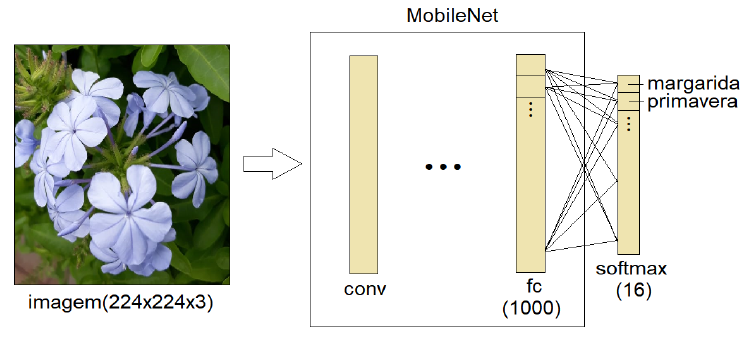
\includegraphics[width=0.8\textwidth]{img/model1.png}
      			\end{center}
      			\caption{Esquema do primeiro modelo proposto. Fonte: elaborada pelo autor.}
  				%\label{fig:birds}
      		\end{figure}
      \end{itemize}
    \end{frame}
    
    \begin{frame}[t]
      \frametitle{Desenvolvimento}
      \framesubtitle{Atividades realizadas}      
      \begin{itemize}
        \item<1-> Alterações realizadas: Modelo 2
        		 \begin{figure}[hbt]
      		 	\begin{center}
      				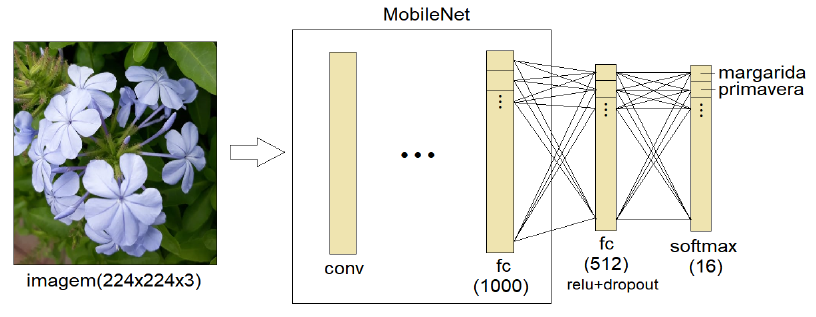
\includegraphics[height=0.35\textwidth]{img/model2.png}
      			\end{center}
      			    \caption{Esquema do segundo modelo proposto. Fonte: elaborada pelo autor.}
      		\end{figure}
      \end{itemize}
    \end{frame}
    
    \begin{frame}[t]
      \frametitle{Desenvolvimento}
      \framesubtitle{Atividades realizadas}      
      \begin{itemize}
        \item<1-> Resumo das alterações: \medskip
        \begin{figure}[hbt]
      		 	\begin{center}
      				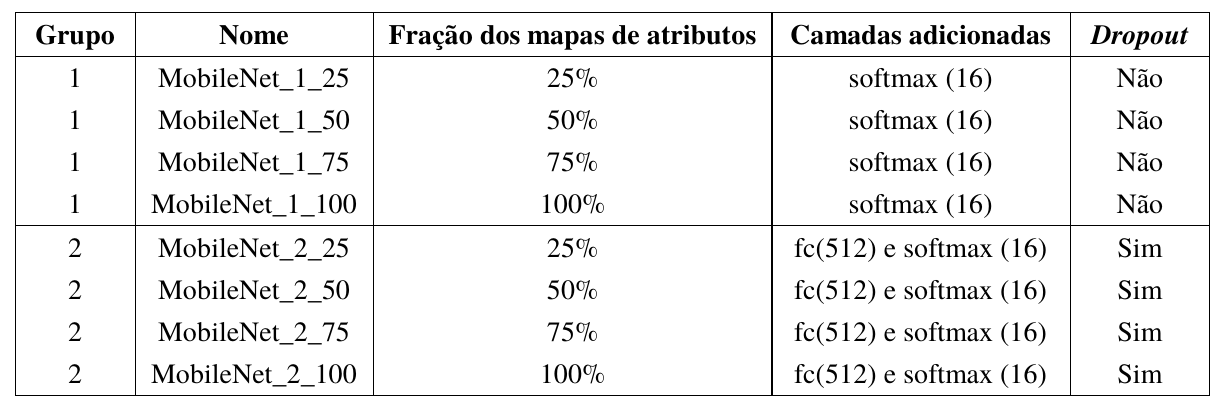
\includegraphics[height=.3 \textwidth]{img/models_table.png}
      			\end{center}
      			\caption{Modelos de rede testados e suas características. Fonte: elaborada pelo autor.}
      		\end{figure}
      \end{itemize}
    \end{frame}
    
    \begin{frame}[t]
      \frametitle{Desenvolvimento}
      \framesubtitle{Atividades realizadas}      
      \begin{itemize}
        \item<1-> Treinamento dos modelos propostos: \medskip
		 \begin{itemize}
        		\item<1-> Lotes de 100 imagens aleatórias; \medskip
        		\item<1-> 5000 iterações; \medskip
        		\item<1-> Acompanhamento em tempo real pela TensorBoard. \medskip
		\end{itemize}        
        \item<2-> Implementação do aplicativo.\medskip
        \begin{itemize}
        		\item<2-> Android Studio;\medskip
        		\item<2-> Versionamento com Git;\medskip
        		\item<2-> Banco de dados orientado a objetos Realm.\medskip
        \end{itemize}
      \end{itemize}
    \end{frame}
        
    %%%%%%%%
    
    \begin{frame}[t]
      \frametitle{Desenvolvimento}
      \framesubtitle{Resultados e Discussão}  \medskip  
      	Treinamentos e arquitetura escolhida \medskip    
      	\begin{itemize}
      		\item Grupo 1
		\end{itemize}      	  	
		\begin{figure}[t]
      		 \begin{minipage}[h]{1.0\linewidth}
         		\centering
      			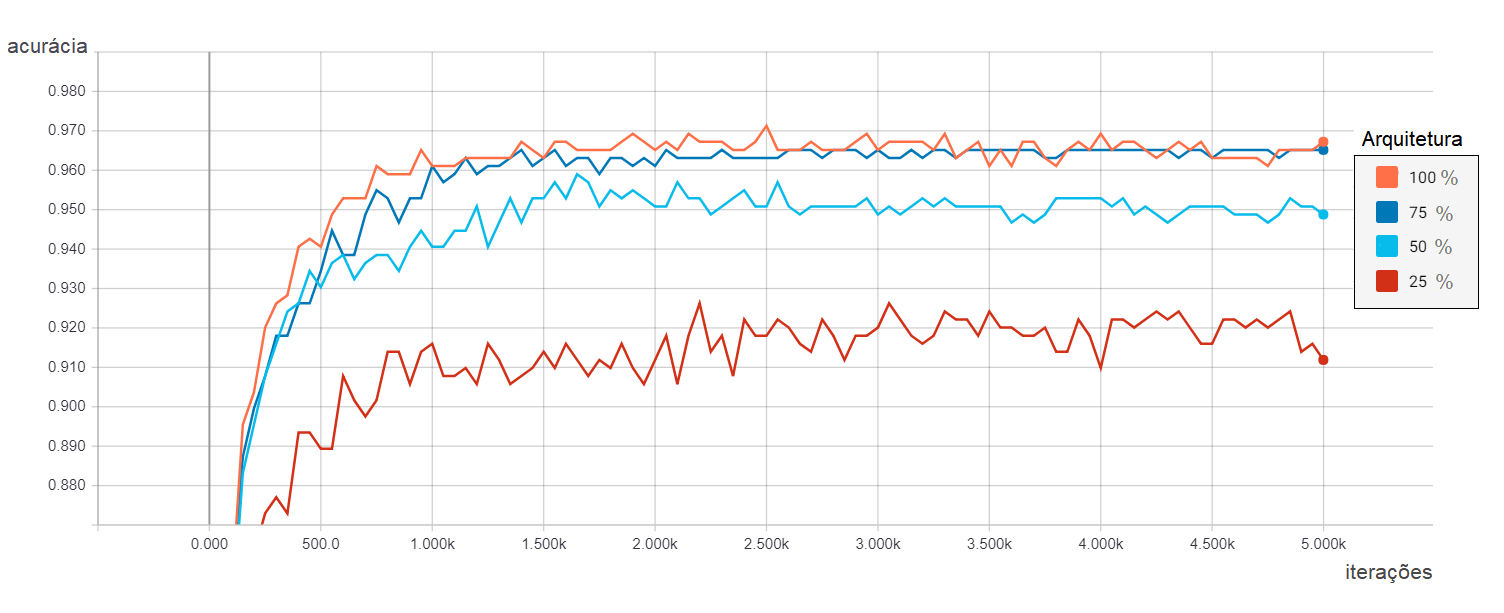
\includegraphics[height=0.42\linewidth]{img/acc_1_5000.png}
      			\caption{Acurácia das redes do grupo 1, no conjunto de validação, ao longo do treinamento.}
      		\end{minipage}
      		\vspace{0.00mm}
      	\end{figure}	      	       
    \end{frame}
    
    \begin{frame}[t]
      \frametitle{Desenvolvimento}
      \framesubtitle{Resultados e Discussão} \medskip       
      	Treinamentos e arquitetura escolhida \medskip    
      	\begin{itemize}
      		\item Grupo 2
		\end{itemize}      	  	
		\begin{figure}[t]
      		 \begin{minipage}[h]{1.0\linewidth}
         		\centering
      			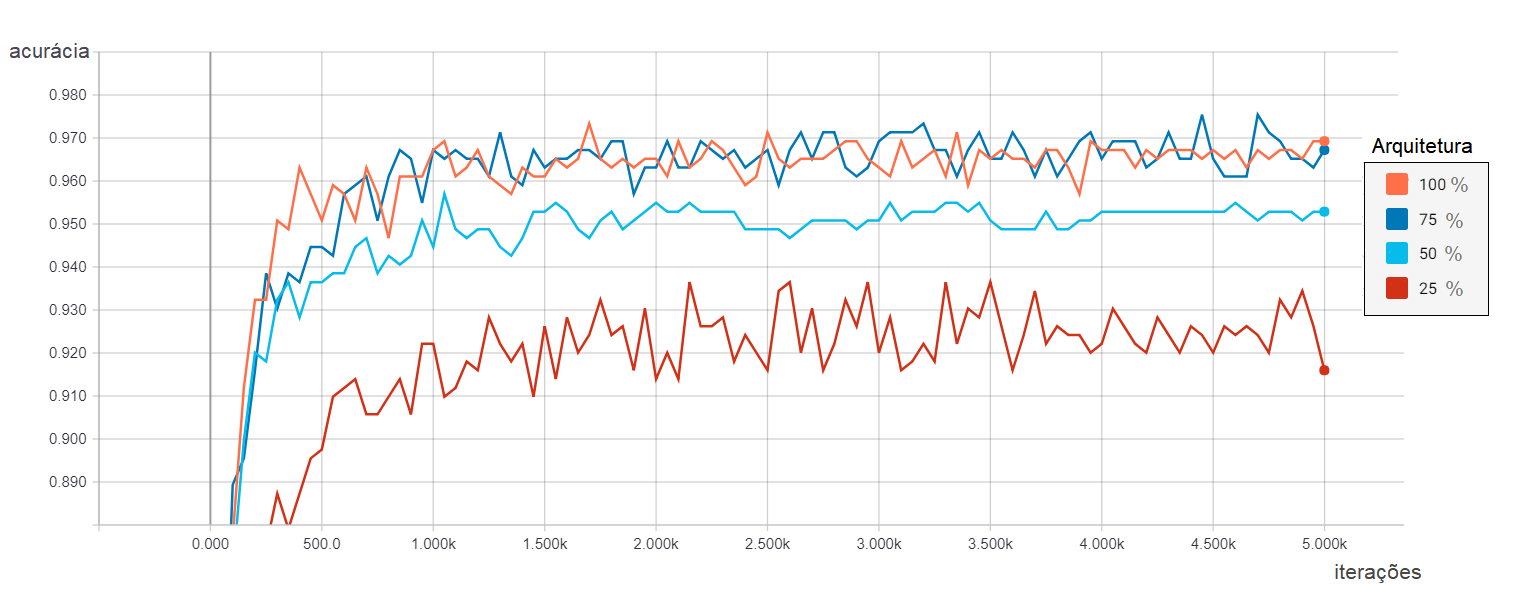
\includegraphics[height=0.42\linewidth]{img/acc_2_5000.png}
      			\caption{Acurácia das redes do grupo 2, no conjunto de validação, ao longo do treinamento.}
      		\end{minipage}
      		\vspace{0.00mm}
      	\end{figure}	      	       
    \end{frame}
    
    \begin{frame}[t]
    		\frametitle{Desenvolvimento}
    		\framesubtitle{Resultados e Discussão}
       	Treinamentos e arquitetura escolhida \medskip    
    		\begin{itemize}
      		\item Maiores valores de acurácia para:
			\begin{itemize}
				\item Grupo 1: MobileNet\_1\_75 e MobileNet\_1\_100
				\item Grupo 2: MobileNet\_2\_75 e MobileNet\_2\_100 \medskip
			\end{itemize}	      		
		\end{itemize}		
		\visible<2->
		{
			Avaliação das duas melhores arquiteturas de cada grupo no conjunto de teste:
			\visible<3->
			{
				\begin{figure}[hbt]
      	 		\begin{center}
      			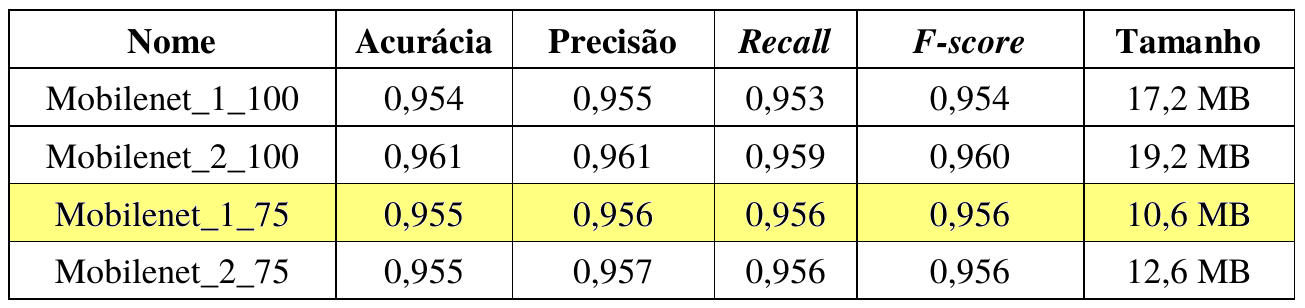
\includegraphics[height=.2 \textwidth]{img/all_metrics_2.png}
      			\end{center}
      			\caption{Valores de acurácia, precisão, recall, F-score e tamanho das arquiteturas escolhidas.}
      			\end{figure}	
			}
		}       	      	
    \end{frame}
	
	\begin{frame}[t]
    		\frametitle{Desenvolvimento}
    		\framesubtitle{Resultados e Discussão}		
		Aplicativo
		\begin{figure}[hbt]
      	 		\begin{center}
      			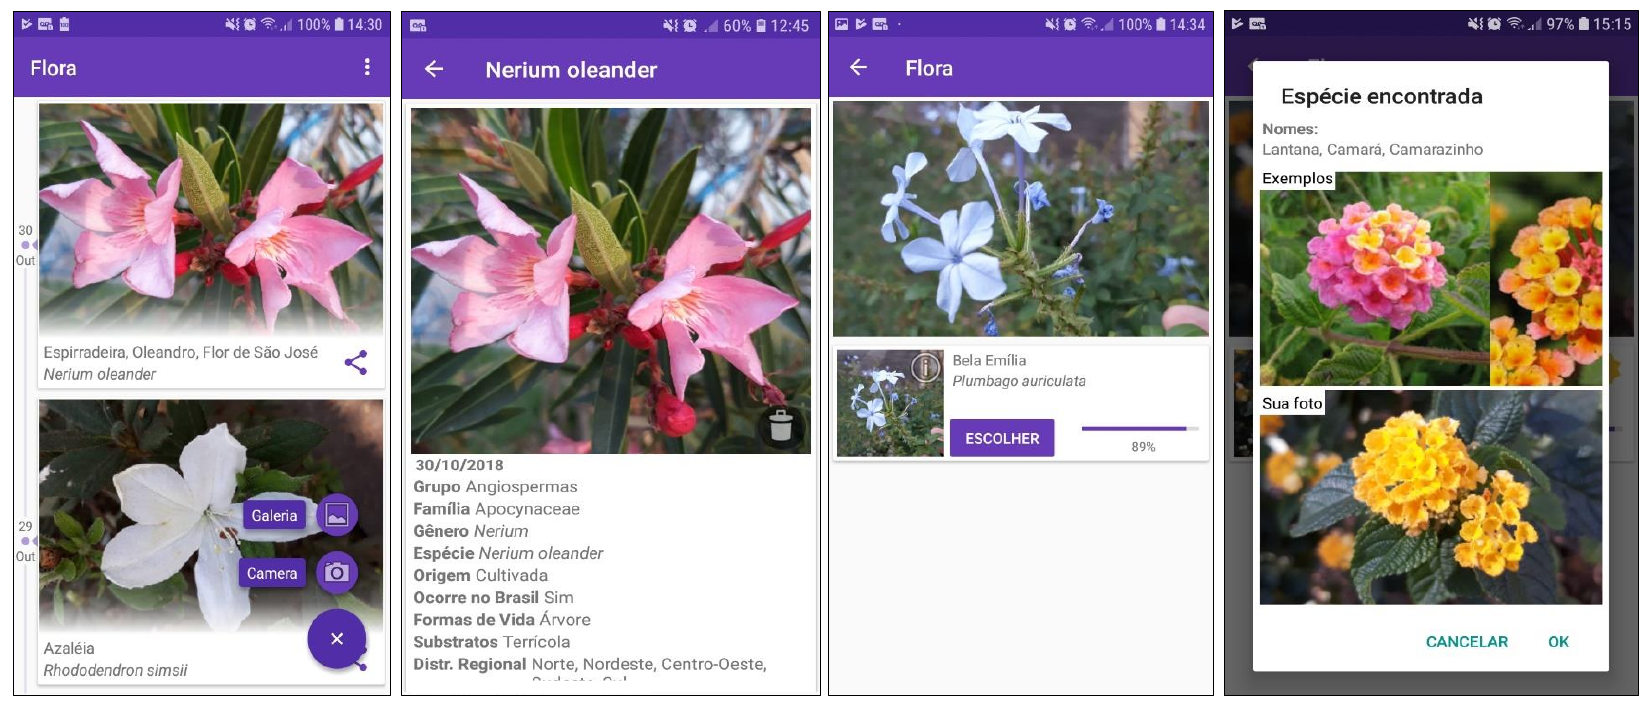
\includegraphics[height=.45 \textwidth]{img/print1.png}
      			\end{center}
      			\caption{Capturas de tela do aplicativo. Fonte: elaborada pelo autor.}
      			\end{figure}	
    \end{frame}  
    
    \begin{frame}[t]
    		\frametitle{Desenvolvimento}
    		\framesubtitle{Resultados e Discussão}		
		Aplicativo \medskip
		\begin{center}
			 \movie{
\includegraphics[width=10.5cm,height=6cm]{img/play.png}}{video/video_tcc.mp4}
		\end{center}
    \end{frame}
    
    %%%%%%%%%%%%%%%%%%%%%%%%%%%% Conclusão
    \section{Conclusão}
      \begin{frame}[t]
      \frametitle{Conclusão}
      Contribuições:
      \begin{itemize} \medskip
      	\item<1-> Confirmação da possibilidade de reutilização, refinamento e manipulação de modelos de redes neurais convolucionais, pré-treinados, para classificação de imagens aplicadas a um contexto mais específico.
		\item<2-> Demonstração da utilização, em ambiente Android, do modelo treinado, através de um aplicativo que pode ser usado por qualquer pessoa. \medskip
		\item<3-> Colaboração da difusão de conhecimentos de botânica. \medskip
      \end{itemize}       
        
    \end{frame}
    
    \begin{frame}[t]
      \frametitle{Conclusão}
      Dificuldades e Limitações:
      \begin{itemize}
        \item<1-> Indisponibildade de hardware (GPU) para treinamento mais rápido das redes, o que inviabilizou 
        a experimentação de diversos parâmetros;
        \item<2-> Ocorrência de erros na execução da rede no aplicativo devido à mudança de linguagem (Python $\rightarrow${} Java);
	    \item<3-> Conjunto de dados limitado.  
      \end{itemize}
      
      \bigskip    
      \visible<4->
      {
      	Trabalhos futuros:
     	\begin{itemize}
        	\item<4-> Treinamento de camadas de convolução e aumento do conjunto de dados e do número de classes;
        	\item<5-> Colaboração do usuário na expansão do conjunto de dados.
      	\end{itemize}
      }
      
    \end{frame}
    
    %%%%%%%%
        
    %%%%%%%%%%%%%%%%%%%%%%%%%%%%
    \section{Referências}   
    \begin{frame}[allowframebreaks]
      \frametitle{Referência Bibliográfica}
      \setbeamertemplate{bibliography item}[text]
      \setbeamercolor{bibliography entry author}{fg=black}
      \setbeamercolor{bibliography item}{fg=black}
      \bibliographystyle{siam}      
      \bibliography{referencias}

    \end{frame}
    
    %%%%%%%%%%%%%%%%%%%%%%%%%%%%
    
    \begin{frame}
        \frametitle{Obrigado!}
        \framesubtitle{Dúvidas?}
        \vskip -\baselineskip
        \vskip -0.55cm \hskip -0.55cm
        \begin{center}
          \maketitle
          \Large{\inserttitle} \\
          \insertauthor \\
          \footnotesize{\insertinstitute}
        \end{center}
    \end{frame}
    

\end{document}
